

\section{Capitulo 4: Implementación de Técnicas UNS en la Plataforma IIoT}
La implementación del UNS en la plataforma de entrenamiento IIoT se basa en la aplicación de técnicas de diseño previamente estudiadas en un entorno académico. Esta aplicación integra sistemas y dispositivos mediante el protocolo MQTT Sparkplug B, estableciendo un modelo jerárquico y estructurado de comunicación orientado a la gestión eficiente de datos.

Este entorno de entrenamiento simula escenarios operacionales reales de la industria  permitiendo a los usuarios interactuar directamente con dispositivos IIoT y validar los principios del UNS en tiempo real.


\subsection{Descripción de la Plataforma IIoT}
La construcción de la plataforma IIoT para entrenamiento en tecnologías de la Industria 4.0 surge como resultado de dos proyectos de investigación estratégicos. El primero, desarrollado bajo la Convocatoria interna VIE en 2021, llevó por título "Plataforma IIoT para formación de profesionales en tecnologías de la cuarta revolución industrial" y se ejecutó entre noviembre de 2021 y noviembre de 2023. Posteriormente, el proyecto "Diseño, desarrollo e implementación de una plataforma IIoT para formación de profesionales en tecnologías de la cuarta revolución industrial", financiado por la Convocatoria 890 de Minciencias, inició en abril de 2023 y se encuentra actualmente en desarrollo. 


\subsubsection{Dispositivos y Nodos Industriales:}
La plataforma se compone de tres casos de estudio, cada uno asociado a un grupo de investigación y con aplicaciones específicas en entornos industriales y académicos:


\begin{itemize}
    \item \textbf{VIVERO:} Pertenece al Grupo de Investigación CENIVAM, donde se monitorean condiciones ambientales dentro de un invernadero mediante un PLC Opto22 - Groov RIO conectado a un termohigrómetro que captura datos de temperatura y humedad. Estos datos son procesados por un servidor Ignition Edge para ser transmitidos.

    \item \textbf{CASIRI:} Pertenece a los Grupos de Investigación RADIOGIS y CEMOS, consiste en una estación de radioastronomía equipada con sensores ambientales que miden temperatura, humedad, presión atmosférica, velocidad y dirección del viento; además de  una cámara multi-espectral para captura de imágenes espectrales y un dispositivo de monitoreo del espectro radioeléctrico. Todos estos dispositivos están integrados mediante un servidor que envía los datos al servidor central.

    \item \textbf{MICRORRED:} Pertenece al Grupo de Investigación GISEL, ubicada en el Laboratorio de Investigación Eléctrica (LIE) en la sede UIS Guatiguara. Este sistema monitorea parámetros críticos de la red eléctrica como tensión RMS, corriente RMS, factor de potencia y diferentes tipos de potencia (aparente, activa y reactiva) mediante un PLC Opto22 - Groov EPIC que utiliza un servidor de Ignition Edge para  prestar servicios a los usuarios.

\end{itemize}

\begin{figure}[h]
\centerline{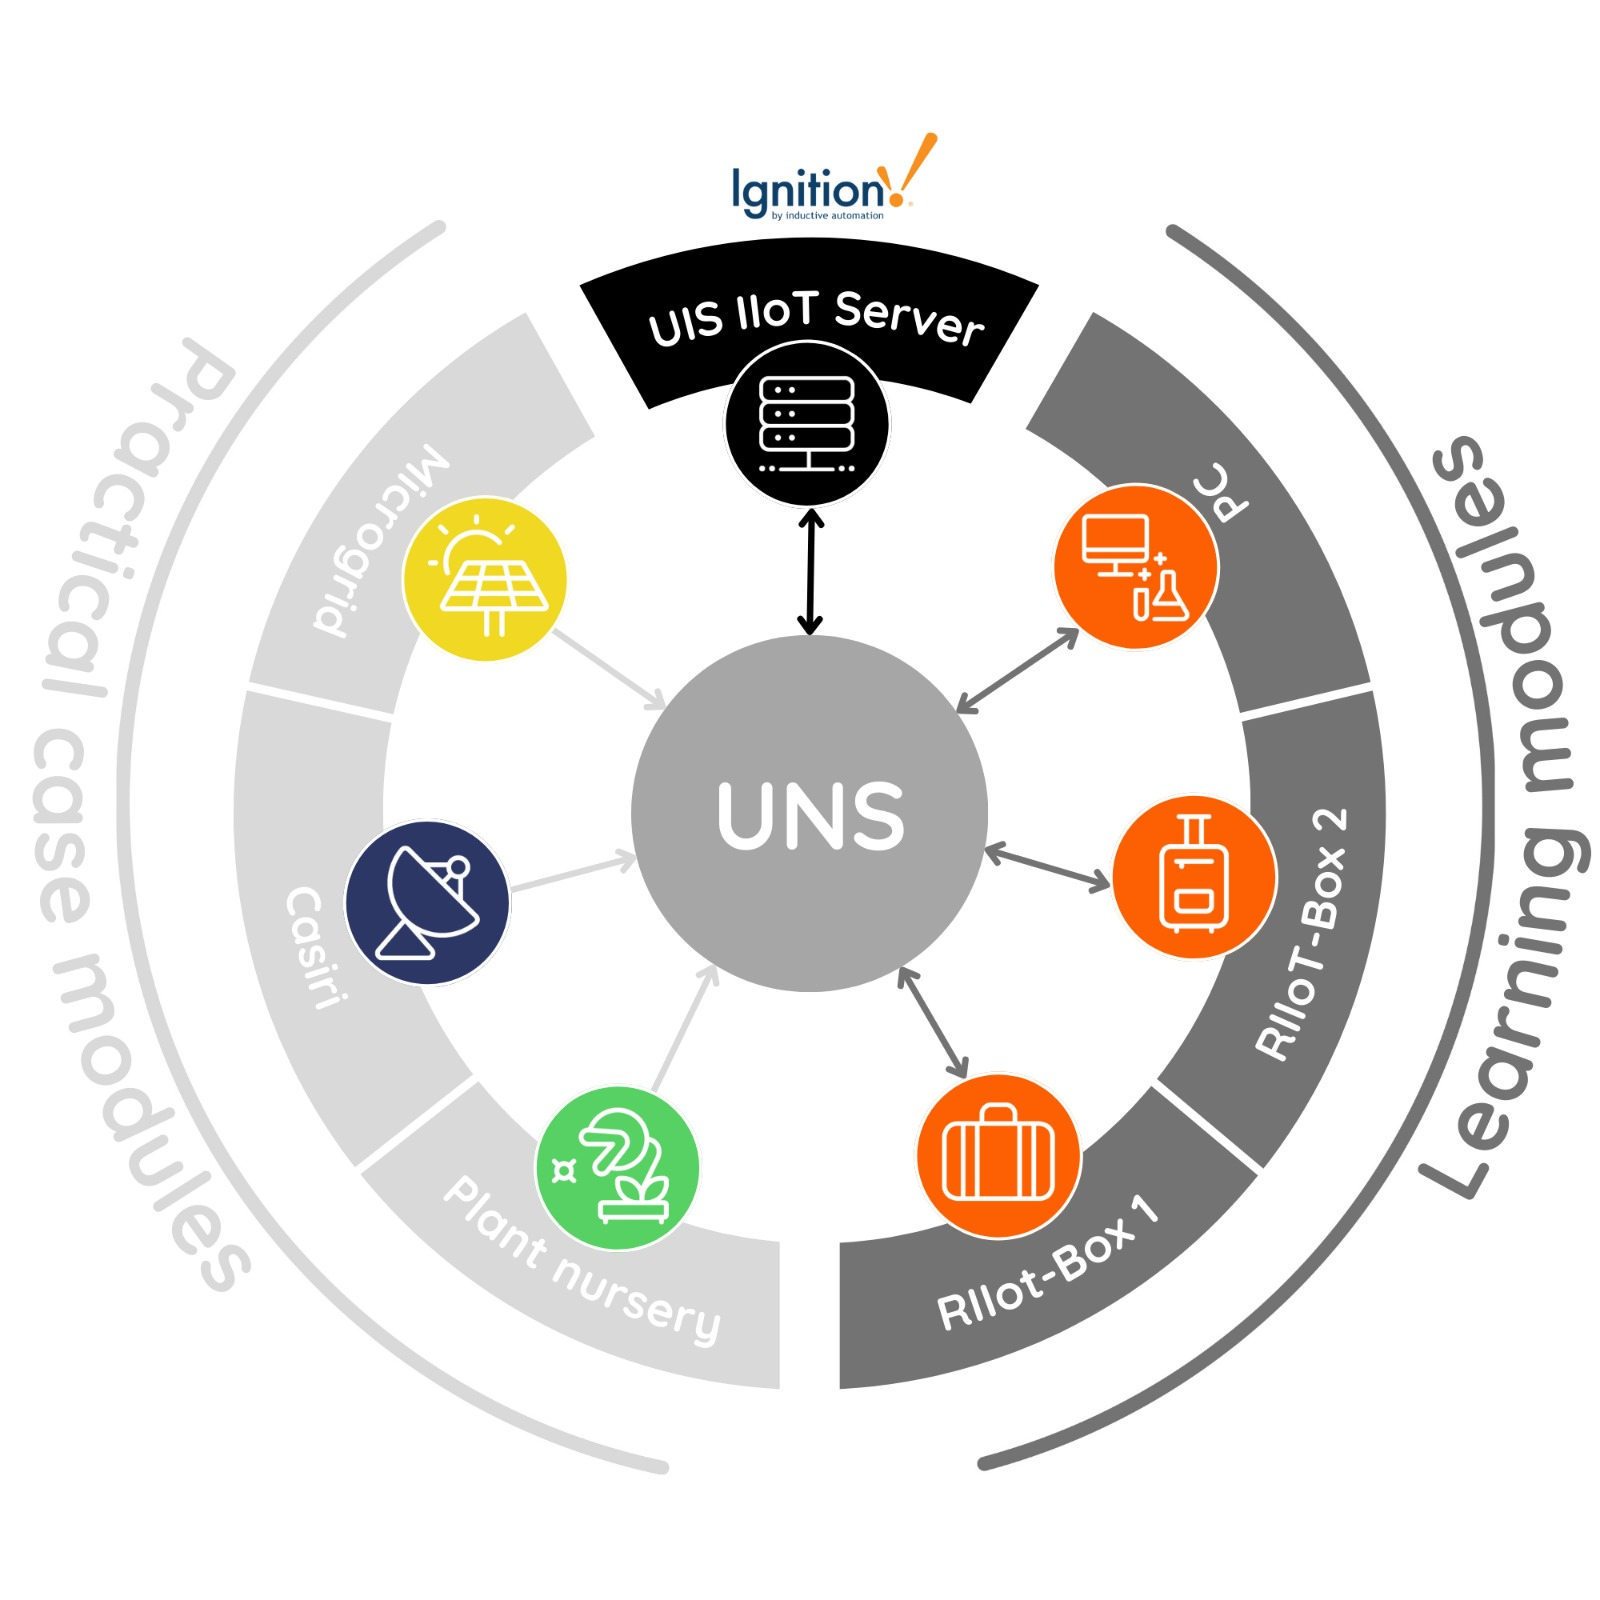
\includegraphics[width=10cm]{Figuras/IIoTPlatform_V2}}
\caption{Esquema de la Plataforma de Entrenamiento IIoT}
\label{fig:iiot_platform}
\end{figure}


Para centralizar la comunicación y visualización de datos en tiempo real de todos los dispositivos (casos de estudio) que actualmente se conectan de forma distribuida a través de internet, se propone implementar un UNS que sea el nodo central del sistema representado en la Figura \ref{fig:iiot_platform}. Allí se debe integrar un broker MQTT escalable a nivel de Enterprise mediante un servidor IIoT, con el objetivo de normalizar los datos, unificar protocolos y gestionar usuarios, permitiendo así una plataforma única para agregar, procesar y visualizar toda la información de los casos de estudio.\\

A partir de la conexión y configuración de los casos de estudio, es posible diseñar un UNS empleando las diversas técnicas de diseño previamente estudiadas y analizadas. Para cada caso, se define un \textit{namespace} estructurado, asegurando una organización eficiente de los datos y su interoperabilidad dentro del sistema.

Ambas metodologías se implementan utilizando el protocolo de comunicación MQTT Sparkplug B, lo que permite la integración de los casos de estudio al servidor principal de manera independiente. A continuación, se detalla el proceso de configuración en la plataforma.


\subsection{Implementación del Método Schultz}

Para la implementación de la técnica de Schultz, se establecen los niveles jerárquicos del UNS, organizando la arquitectura del sistema en función de los \textit{sites, areas, lines y cells} como se adquieren los datos. Esta estructura permite una gestión eficiente de la información para la integración de los dispositivos en la plataforma de entrenamiento IIoT.

El sistema está compuesto por dos \textit{sites} principales: Central y Guatiguará. En el \textit{site} Central, se encuentran dos \textit{areas} diferenciadas. La primera, Cenivam, comprende la \textit{line} Vivero y la \textit{cell} GroovRio, donde este último es el PLC encargado de la adquisición de datos a través del termo-higrómetro. La segunda \textit{area}, Radiogis, está conformada por la \textit{line} Casiri, las \textit{cell} Cámara, responsables de la captura de imágenes espectrales, y la \textit{cell} Estación Ambiental, que recopila información sobre variables ambientales.

Por otro lado, en el \textit{site} Guatiguará, se encuentra el \textit{area} LIE (Laboratorio de Integración Energética), la cual alberga la \textit{line} Microrred y la \textit{cell} GroovEpic, un PLC encargado de la adquisición de datos eléctricos de la Microrred.


\subsubsection{Arquitectura de Diseño}

Para implementar esta técnica en la aplicación de Ignition basada en MQTT Sparkplug B, se diseña la arquitectura mostrada en la Fig. \ref{fig:arqIIoT_Schultz}, en donde se escala desde el nivel de \textit{area}, al nivel de  \textit{site} y finalmente al nivel de \textit{Enterprise}.

\begin{figure}[H]
\centerline{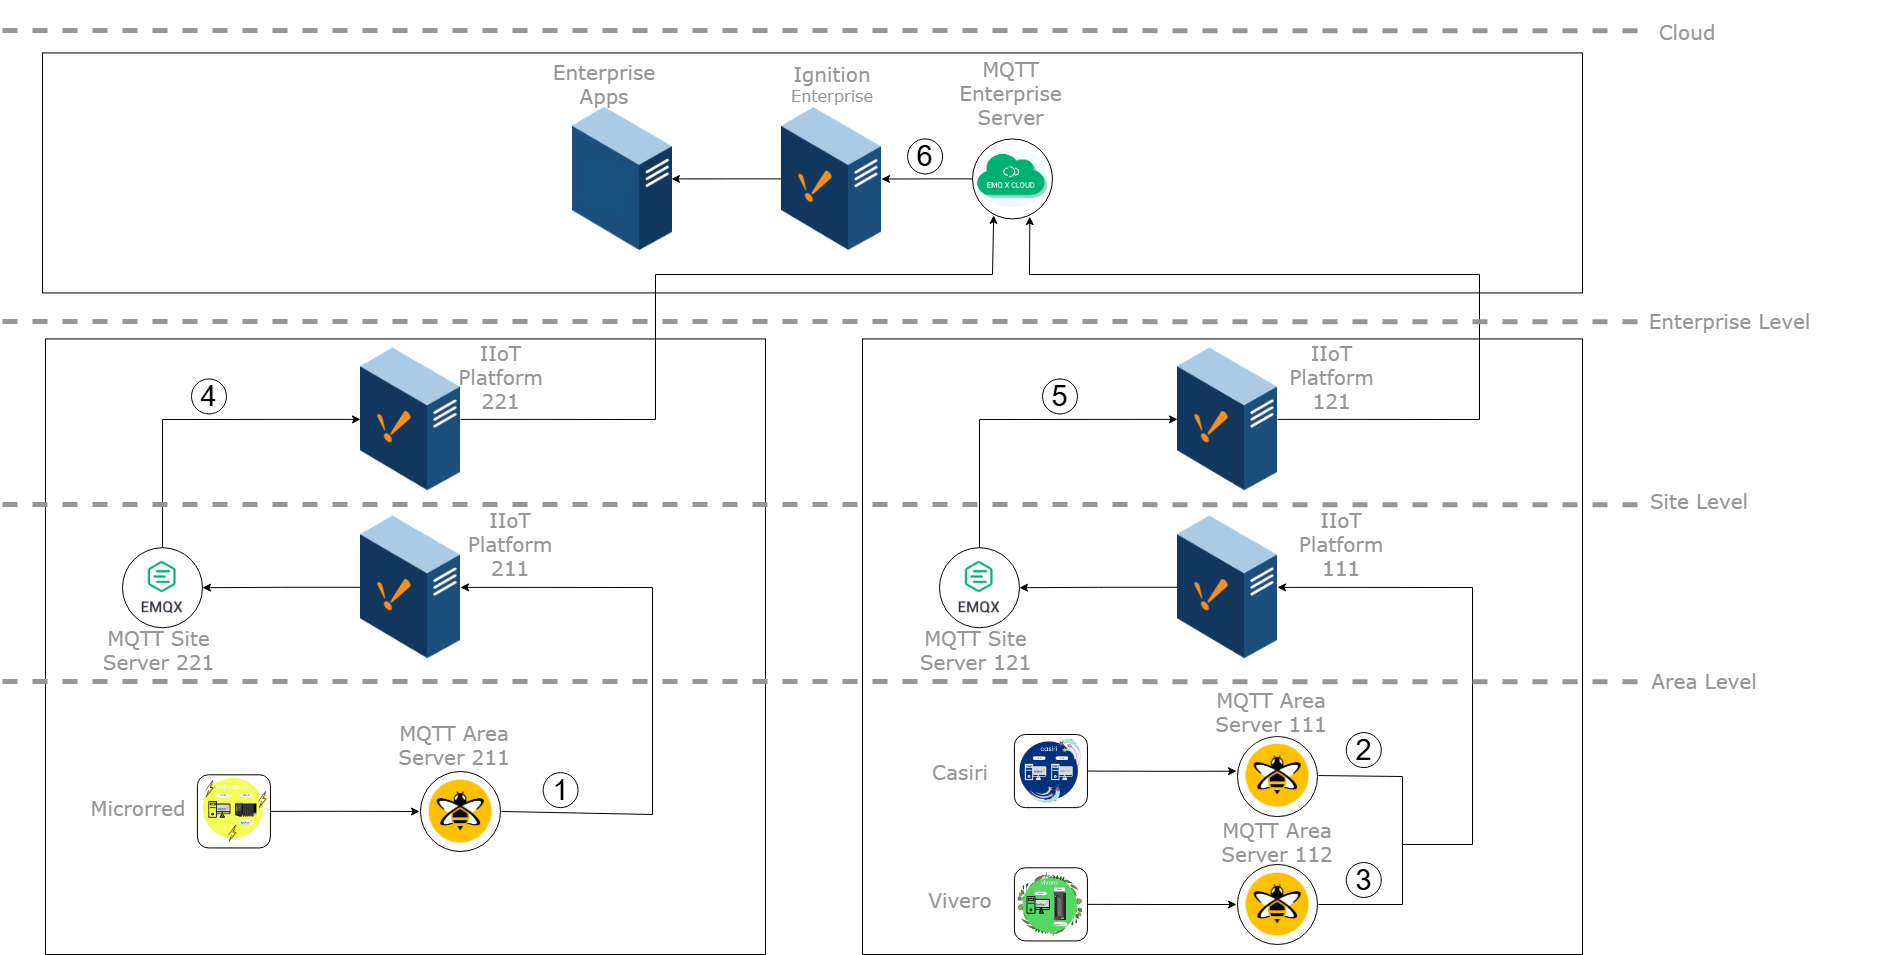
\includegraphics[width=19cm]{Figuras/ArqSchultz_IIoT_V3.png}}
\caption{Esquema de la Arquitectura UNS con el Método de Schultz en la Plataforma IIoT}
\label{fig:arqIIoT_Schultz}
\end{figure}


Los dispositivos IIoT de cada uno de los casos de estudio de la plataforma IIoT, se conectan a brokers de HiveMQ (MQTT Area Server 111, MQTT Area Server 112 y MQTT Site Server 211), que actúan como concentradores de datos para áreas específicas. Estos brokers recogen los datos y los envían a las Plataformas IIoT 111 y 211 para organizar los datos en un UNS de \textit{area} para cada caso, con la siguiente estructura: (\textcircled{1}, \textcircled{2} y \textcircled{3} en Fig. \ref{fig:arqIIoT_Schultz}) 

\begin{figure}[H]
\centering
\begin{minipage}{0.32\textwidth}
\centering
\scalebox{0.7}{
\begin{forest}
  for tree={
    font=\ttfamily,
    grow'=0,
    child anchor=west,
    parent anchor=south,
    anchor=west,
    calign=first,
    edge path={
      \noexpand\path [draw, \forestoption{edge}]
      (!u.south west) +(7.5pt,0) |- node[fill,inner sep=1.25pt] {} (.child anchor)\forestoption{edge label};
    },
    before typesetting nodes={
      if n=1
        {insert before={[,phantom]}}
        {}
    },
    fit=band,
    before computing xy={l=15pt},
  }
[\textbf{Area:} LIE
   [\textbf{Line:} Microrred
    [\textbf{Cell:} GroovEpic]
]
]
\end{forest}
}
\end{minipage}%
\begin{minipage}{0.32\textwidth}
\centering
\scalebox{0.7}{
\begin{forest}
  for tree={
    font=\ttfamily,
    grow'=0,
    child anchor=west,
    parent anchor=south,
    anchor=west,
    calign=first,
    edge path={
      \noexpand\path [draw, \forestoption{edge}]
      (!u.south west) +(7.5pt,0) |- node[fill,inner sep=1.25pt] {} (.child anchor)\forestoption{edge label};
    },
    before typesetting nodes={
      if n=1
        {insert before={[,phantom]}}
        {}
    },
    fit=band,
    before computing xy={l=15pt},
  }
[\textbf{Area:} Radiogis
   [\textbf{Line:} Casiri
    [\textbf{Cell:} Camara]
    [\textbf{Cell:} Estacion Ambiental]
]
]
\end{forest}
}
\end{minipage}%
\begin{minipage}{0.32\textwidth}
\centering
\scalebox{0.7}{
\begin{forest}
  for tree={
    font=\ttfamily,
    grow'=0,
    child anchor=west,
    parent anchor=south,
    anchor=west,
    calign=first,
    edge path={
      \noexpand\path [draw, \forestoption{edge}]
      (!u.south west) +(7.5pt,0) |- node[fill,inner sep=1.25pt] {} (.child anchor)\forestoption{edge label};
    },
    before typesetting nodes={
      if n=1
        {insert before={[,phantom]}}
        {}
    },
    fit=band,
    before computing xy={l=15pt},
  }
[\textbf{Area:} Cenivam
   [\textbf{Line:} Vivero
    [\textbf{Cell:} GroovRio]
]
]
\end{forest}
}
\end{minipage}
\end{figure}


%\begin{figure}[H] 
\centering
\scalebox{0.7}{
\begin{forest}
  for tree={
    font=\ttfamily,
    grow'=0,
    child anchor=west,
    parent anchor=south,
    anchor=west,
    calign=first,
    edge path={
      \noexpand\path [draw, \forestoption{edge}]
      (!u.south west) +(7.5pt,0) |- node[fill,inner sep=1.25pt] {} (.child anchor)\forestoption{edge label};
    },
    before typesetting nodes={
      if n=1
        {insert before={[,phantom]}}
        {}
    },
    fit=band,
    before computing xy={l=15pt},
  }
[\textbf{Area:} LIE
   [\textbf{Line:} Microrred
    [\textbf{Cell:} GroovEpic]
]
]
\end{forest}
}

\end{figure}

%\begin{figure}[H] 
\centering
\scalebox{0.7}{
\begin{forest}
  for tree={
    font=\ttfamily,
    grow'=0,
    child anchor=west,
    parent anchor=south,
    anchor=west,
    calign=first,
    edge path={
      \noexpand\path [draw, \forestoption{edge}]
      (!u.south west) +(7.5pt,0) |- node[fill,inner sep=1.25pt] {} (.child anchor)\forestoption{edge label};
    },
    before typesetting nodes={
      if n=1
        {insert before={[,phantom]}}
        {}
    },
    fit=band,
    before computing xy={l=15pt},
  }
[\textbf{Area:} Radiogis
   [\textbf{Line:} Casiri
    [\textbf{Cell:} Camara]
    [\textbf{Cell:} Estacion Ambiental]
]
]
\end{forest}
}

\end{figure}

%\begin{figure}[H] 
\centering
\scalebox{0.7}{
\begin{forest}
  for tree={
    font=\ttfamily,
    grow'=0,
    child anchor=west,
    parent anchor=south,
    anchor=west,
    calign=first,
    edge path={
      \noexpand\path [draw, \forestoption{edge}]
      (!u.south west) +(7.5pt,0) |- node[fill,inner sep=1.25pt] {} (.child anchor)\forestoption{edge label};
    },
    before typesetting nodes={
      if n=1
        {insert before={[,phantom]}}
        {}
    },
    fit=band,
    before computing xy={l=15pt},
  }
[\textbf{Area:} Cenivam
   [\textbf{Line:} Vivero
    [\textbf{Cell:} GroovRio]
]
]
\end{forest}
}

\end{figure}


Secuencialmente, los UNS de \textit{area} son enviados a un broker local (MQTT Site Server 121 y 221) para recolectar la información por \textit{site} y enviarlas a las Plataformas IIoT 121 y 221. Estas procesan los datos contextualizados y organizan los datos en un UNS de \textit{site} con la siguiente estructura:(\textcircled{4} y  \textcircled{5} en Fig. \ref{fig:arqIIoT_Schultz}))\\

\begin{figure}[H]
\centering
\begin{minipage}{0.32\textwidth}
\centering
\scalebox{0.6}{
\begin{forest}
  for tree={
    font=\ttfamily,
    grow'=0,
    child anchor=west,
    parent anchor=south,
    anchor=west,
    calign=first,
    edge path={
      \noexpand\path [draw, \forestoption{edge}]
      (!u.south west) +(7.5pt,0) |- node[fill,inner sep=1.25pt] {} (.child anchor)\forestoption{edge label};
    },
    before typesetting nodes={
      if n=1
        {insert before={[,phantom]}}
        {}
    },
    fit=band,
    before computing xy={l=15pt},
  }
  [\textbf{Site:} Guatiguara  
    [\textbf{Area:} LIE
       [\textbf{Line:} Microrred
        [\textbf{Cell:} GroovEpic]
       ]
    ]
  ]
\end{forest}
}
\end{minipage}%
\begin{minipage}{0.32\textwidth}
\centering
\scalebox{0.6}{
\begin{forest}
  for tree={
    font=\ttfamily,
    grow'=0,
    child anchor=west,
    parent anchor=south,
    anchor=west,
    calign=first,
    edge path={
      \noexpand\path [draw, \forestoption{edge}]
      (!u.south west) +(7.5pt,0) |- node[fill,inner sep=1.25pt] {} (.child anchor)\forestoption{edge label};
    },
    before typesetting nodes={
      if n=1
        {insert before={[,phantom]}}
        {}
    },
    fit=band,
    before computing xy={l=15pt},
  }
[\textbf{Site:} Central
    [\textbf{Area:} Radiogis
       [\textbf{Line:} Casiri
        [\textbf{Cell:} Camara]
        [\textbf{Cell:} Estacion Ambiental]
       ]
    ]
    [\textbf{Area:} Cenivam
       [\textbf{Line:} Vivero
        [\textbf{Cell:} GroovRio]
       ]
    ]
]
\end{forest}
}
\end{minipage}
\end{figure}



Finalmente, con la estructura definida para cada uno de los \textit{site}, se consolidan todos los namespaces distribuidos en un broker en la nube (MQTT Enterprise Server). Este recibe todas las áreas de la infraestructura y organiza el UNS a nivel de \textit{Enterprise} en el Ignition Enterprise, con el siguiente modelo jerárquico.(\textcircled{6} en Fig. \ref{fig:arqIIoT_Schultz}) 

\begin{figure}[H] 
\centering
\scalebox{0.7}{
\begin{forest}
  for tree={
    font=\ttfamily,
    grow'=0,
    child anchor=west,
    parent anchor=south,
    anchor=west,
    calign=first,
    edge path={
      \noexpand\path [draw, \forestoption{edge}]
      (!u.south west) +(7.5pt,0) |- node[fill,inner sep=1.25pt] {} (.child anchor)\forestoption{edge label};
    },
    before typesetting nodes={
      if n=1
        {insert before={[,phantom]}}
        {}
    },
    fit=band,
    before computing xy={l=15pt},
  }
[\textbf{Enterprise:} UIS
  [\textbf{Site:} Central
    [\textbf{Area:} Cenivam
        [\textbf{Line:} Vivero
            [\textbf{Cell:} GroovRio]
        ]
    ]
    [\textbf{Area:} Radiogis 
        [\textbf{Line:} Casiri
            [\textbf{Cell:} Camara]
            [\textbf{Cell:} Estacion Ambiental]
        ]
    ]
]
   [\textbf{Site:} Guatiguara
    [\textbf{Area:} LIE
        [\textbf{Line:} Microrred
            [\textbf{Cell:} GroovEpic]
        ]
    ]
]
]
\end{forest}
}

\end{figure}


La nube opera como la capa de integración global, permitiendo analítica avanzada y gestión remota de cada uno de los niveles de la jerarquía, además permite la conexión de diferentes aplicaciones al nivel de \textit{Enterprise} para monitorear y controlar los datos. Esta estructura multi-capa mantiene la autonomía local, evita los diferentes silos de datos y permite la re-conexión automática de los datos ante una falla en el sistema en cualquier nivel del UNS.

\subsubsection{Implementación en Ignition}

Una vez diseñada e implementada la arquitectura del UNS utilizando el método de Schultz, es posible establecer conexión con el servidor Enterprise MQTT a través de la aplicación Ignition. Esta conexión permite visualizar de forma estructurada y en tiempo real toda la jerarquía del UNS previamente definida, facilitando el acceso a los datos organizados por \textit{sites}, \textit{areas}, \textit{lines} y \textit{cells}. La plataforma Ignition actúa como cliente MQTT compatible con Sparkplug B, lo que permite la exploración y supervisión directa del modelo UNS. A continuación, se presenta una visualización dentro del entorno de Ignition.

\begin{figure}[h]
\centerline{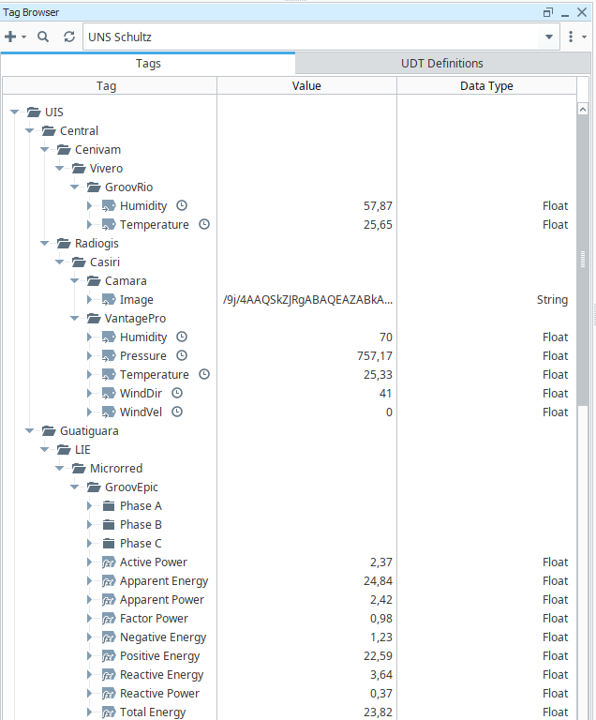
\includegraphics[width=8cm]{Figuras/UNS_Schultz_Ignition}}
\caption{UNS Schultz en Ignition}
\label{fig:unsSchultzig}
\end{figure}

A través de esta estructura jerárquica es posible acceder a los datos de toda la infraestructura, desde el nivel \textit{Enterprise} hasta el nivel de \textit{cell}, reflejando con precisión los distintos niveles definidos en el UNS. Cada uno de estos niveles representa una instancia clara dentro de la jerarquía del sistema, lo que garantiza una organización coherente y uniforme de los dispositivos y sensores conectados en las diferentes áreas.

Esta estandarización en la representación y ubicación de los dispositivos permite lograr una alta escalabilidad e interoperabilidad sin necesidad de modificar la arquitectura base. De esta manera, cualquier nuevo caso de estudio o integración de un dispositivo adicional puede ser incorporado directamente en el área correspondiente, y automáticamente será reflejado en el UNS general, manteniendo la integridad y consistencia del sistema.

\subsection{Implementación del Método Parris}

Para la aplicación de la técnica de Parris en la plataforma IIoT, se define la jerarquía del UNS replicando la estructura utilizada previamente, basada en los mismos \textit{sites}, \textit{areas}, \textit{lines} y \textit{cells} de adquisición de datos de la plataforma. La arquitectura contempla nuevamente dos \textit{sites} principales: Central, que incluye las \textit{areas} Cenivam, con la \textit{line} Vivero y la \textit{cell} GroovRio, además del Radiogis, con la \textit{line} Casiri y las \textit{cells} Cámara y Estación Ambiental; por otro lado, se tiene el \textit{site} Guatiguará, que incorpora el \textit{area} LIE, compuesta por la \textit{line} Microrred y la \textit{cell} GroovEpic.

\subsubsection{Arquitectura de Diseño}

La arquitectura basada en el método de Parris presenta un enfoque simplificado y estandarizado para implementar un UNS, utilizando un broker MQTT centralizado como columna vertebral de la comunicación. A diferencia del modelo jerárquico de Schultz, aquí todos los dispositivos (Sensor 1, Sensor 2, Sensor 3) de los 3 casos de estudios y las aplicaciones (como Ignition Enterprise) se conectan directamente al mismo MQTT Broker en la nube, eliminando capas intermedias de servidores locales. En la Fig. \ref{fig:arqIIoT_Parris} se representa como cada dispositivo publica datos en rutas estandarizadas (UNS Path) para cada uno de los casos, que definen un namespace unificado y accesible para toda la organización. Algunos ejemplos de UNS Path utilizando el delimitador \textit{"\_"} son los siguientes:


\begin{center}
    UNS Path 1: \textit{UIS\_Central/Radiogis\_Casiri\_Estacion Ambiental/<device\_id>}\\
    UNS Path 2: \textit{UIS\_Central/Cenivam\_Vivero\_GroovRio/<device\_id>}\\
    UNS Path 3: \textit{UIS\_Guatiguara/LIE\_Microrred\_GroovEpic/<device\_id>}
\end{center}



\begin{figure}[H]
\centerline{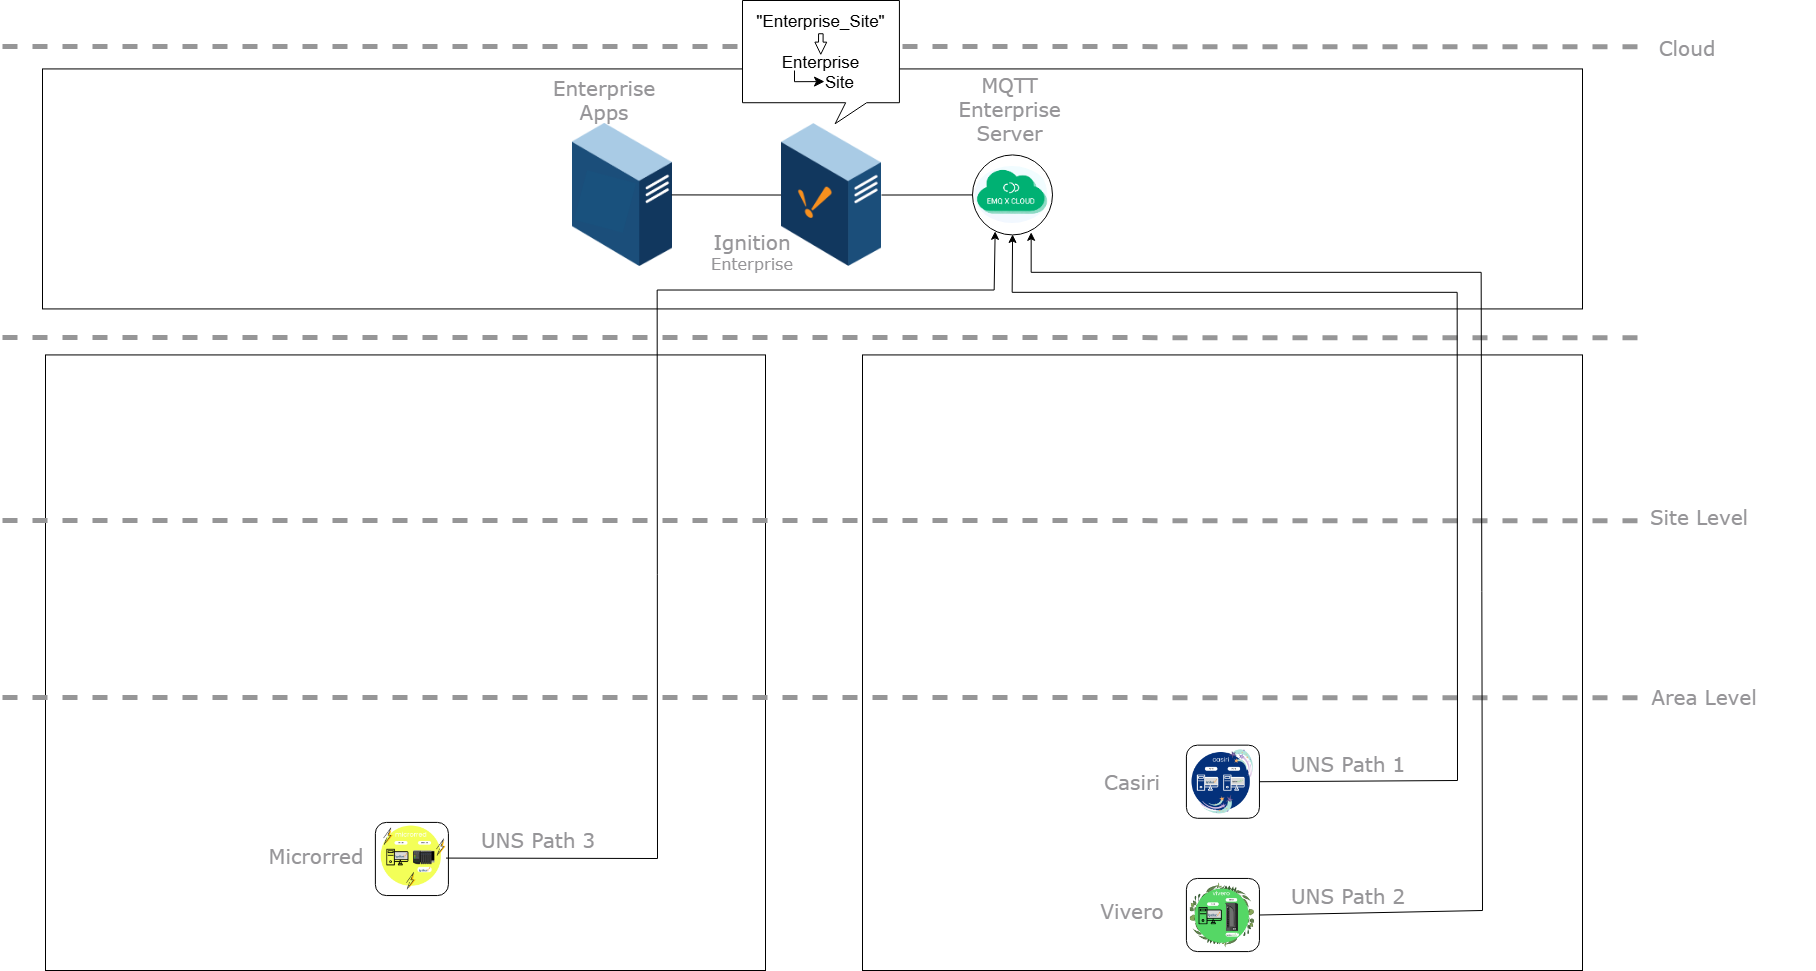
\includegraphics[width=19cm]{Figuras/ArqParris_IIoT_V3.png}}
\caption{Esquema de la Arquitectura UNS con el Metodo de Parris en la Plataforma IIoT}
\label{fig:arqIIoT_Parris}
\end{figure}


Las aplicaciones acceden directamente al broker central para visualizar, analizar y controlar los datos en tiempo real. De manera similar al método de Schultz, la jerarquía del UNS diseñada desde la plataforma Ignition Enterprise se representa con la siguiente estructura.

\begin{figure}[H] 
\centering
\scalebox{0.7}{
\begin{forest}
  for tree={
    font=\ttfamily,
    grow'=0,
    child anchor=west,
    parent anchor=south,
    anchor=west,
    calign=first,
    edge path={
      \noexpand\path [draw, \forestoption{edge}]
      (!u.south west) +(7.5pt,0) |- node[fill,inner sep=1.25pt] {} (.child anchor)\forestoption{edge label};
    },
    before typesetting nodes={
      if n=1
        {insert before={[,phantom]}}
        {}
    },
    fit=band,
    before computing xy={l=15pt},
  }
[\textbf{Enterprise:} UIS
  [\textbf{Site:} Central
    [\textbf{Area:} Cenivam
        [\textbf{Line:} Vivero
            [\textbf{Cell:} GroovRio]
        ]
    ]
    [\textbf{Area:} Radiogis 
        [\textbf{Line:} Casiri
            [\textbf{Cell:} Camara]
            [\textbf{Cell:} Estacion Ambiental]
        ]
    ]
]
   [\textbf{Site:} Guatiguara
    [\textbf{Area:} LIE
        [\textbf{Line:} Microrred
            [\textbf{Cell:} GroovEpic]
        ]
    ]
]
]
\end{forest}
}

\end{figure}



El método de Parris destaca por su simplicidad y flexibilidad, ideal para entornos donde la agilidad y la conectividad directa son prioritarias. Al eliminar servidores intermedios, se reduce el mantenimiento y se acelera la implementación, aunque requiere un broker MQTT robusto y una red confiable para manejar todo el tráfico de datos de manera eficiente.



\subsubsection{Implementación  en Ignition}

Una vez implementada la arquitectura del UNS, se establece la conexión con el broker MQTT centralizado, el cual contiene la estructura completa del sistema. A través de la aplicación Ignition, es posible visualizar cada uno de los ``Paths'' correspondientes a los casos de estudio, estructurados según el delimitador definido. Esta visualización se realiza conforme a la especificación MQTT Sparkplug B, adoptando la siguiente organización jerárquica:

\begin{center}      
    \textit{<group\_id>: Enterprise\_Site}\\ 
    \textit{<edgenode\_id>: Area\_Line\_Cell}\\ 
\end{center}

En la Fig \ref{fig:unsParrisig_engine} se puede observar como se reciben los topics en Ignition según la especificación del protocolo y la definición de cada uno de los nodos.


\begin{figure}[H]
\centerline{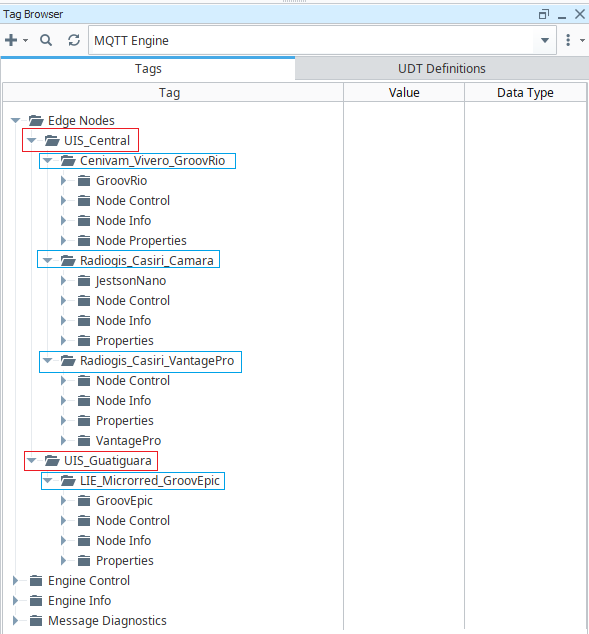
\includegraphics[width=8cm]{Figuras/UNS_Engine_Parris_Ignition_V2}}
\caption{Método de Parris en el Módulo MQTT Engine en Ignition}
\label{fig:unsParrisig_engine}
\end{figure}

La aplicación permite recibir y procesar los ``topics''
suscritos, y como se muestra en la Fig. \ref{fig:unsParrisig}, Ignition interpreta los delimitadores ``\_'' para dividirlos en sub-topics, construyendo así la jerarquía del UNS definida previamente.


\begin{figure}[H]
\centerline{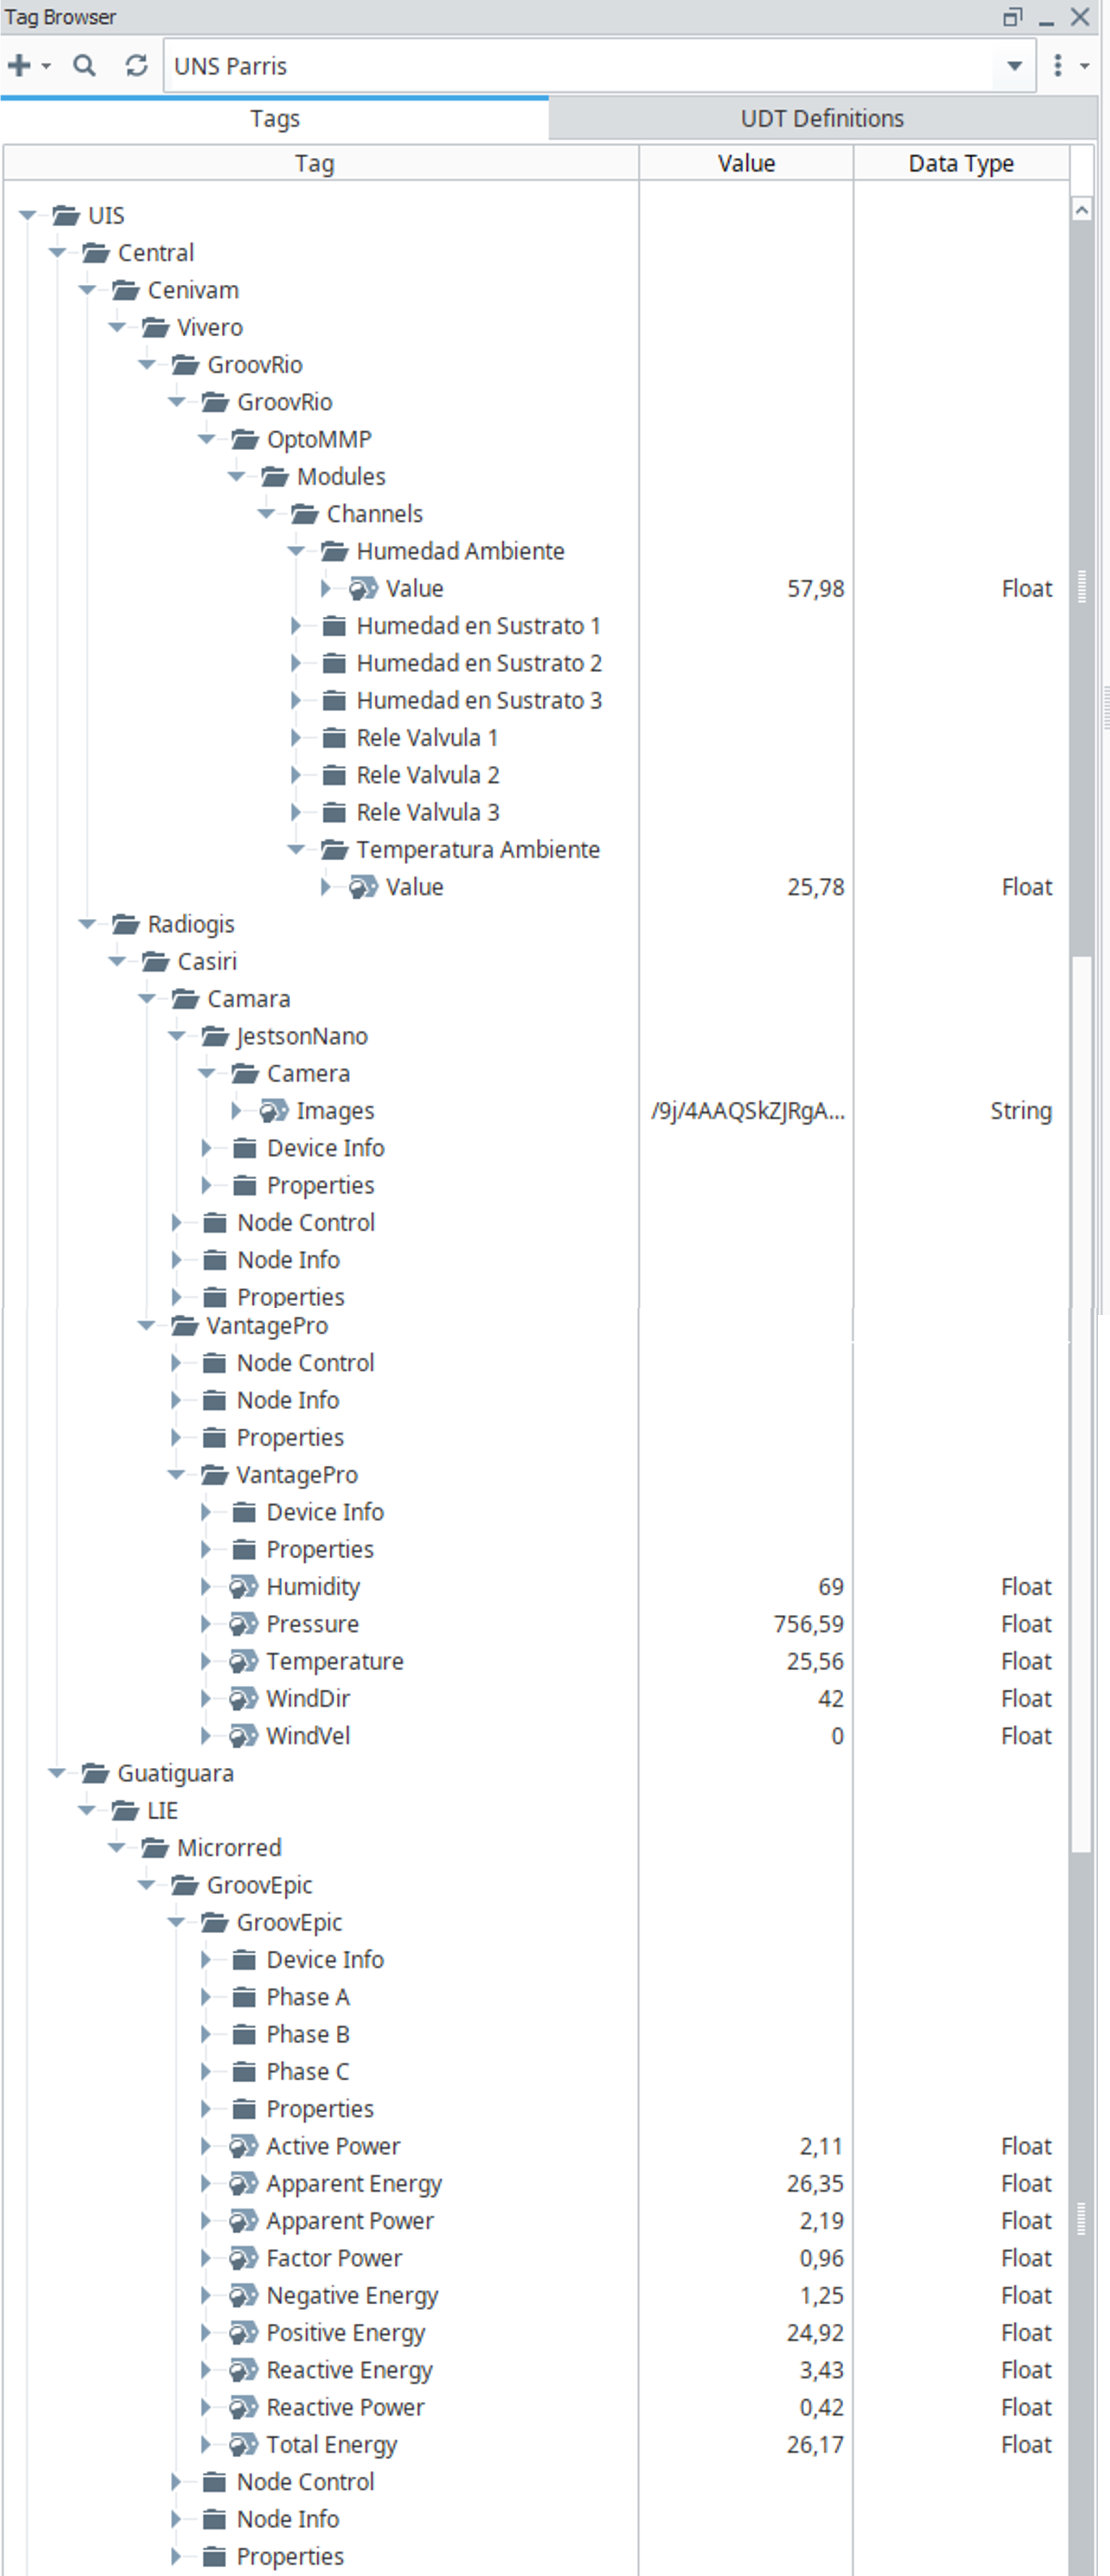
\includegraphics[width=7.9cm]{Figuras/UNS_Parris_Ignition}}
\caption{Método de Parris Estructurado en Ignition}
\label{fig:unsParrisig}
\end{figure}



\subsection{Aplicación Ignition Plataforma IIoT}

La plataforma Ignition actúa como interfaz de visualización dentro de la arquitectura IIoT basada en Unified Namespace, proporcionando al usuario final acceso estructurado a los datos del sistema. En esta etapa, se detalla el diseño del \textit{Front-End} de la aplicación, incluyendo la disposición de vistas, widgets e indicadores interactivos que permiten la supervisión, análisis y control operativo en tiempo real de forma eficiente e intuitiva.

La vista principal de la aplicación corresponde al Home, como se muestra en la Figura \ref{fig:homeUNS}. Esta pantalla centraliza el acceso a los distintos módulos de monitoreo, permitiendo navegar de forma intuitiva entre los distintos sites y componentes del sistema.

\begin{figure}[H]
\centerline{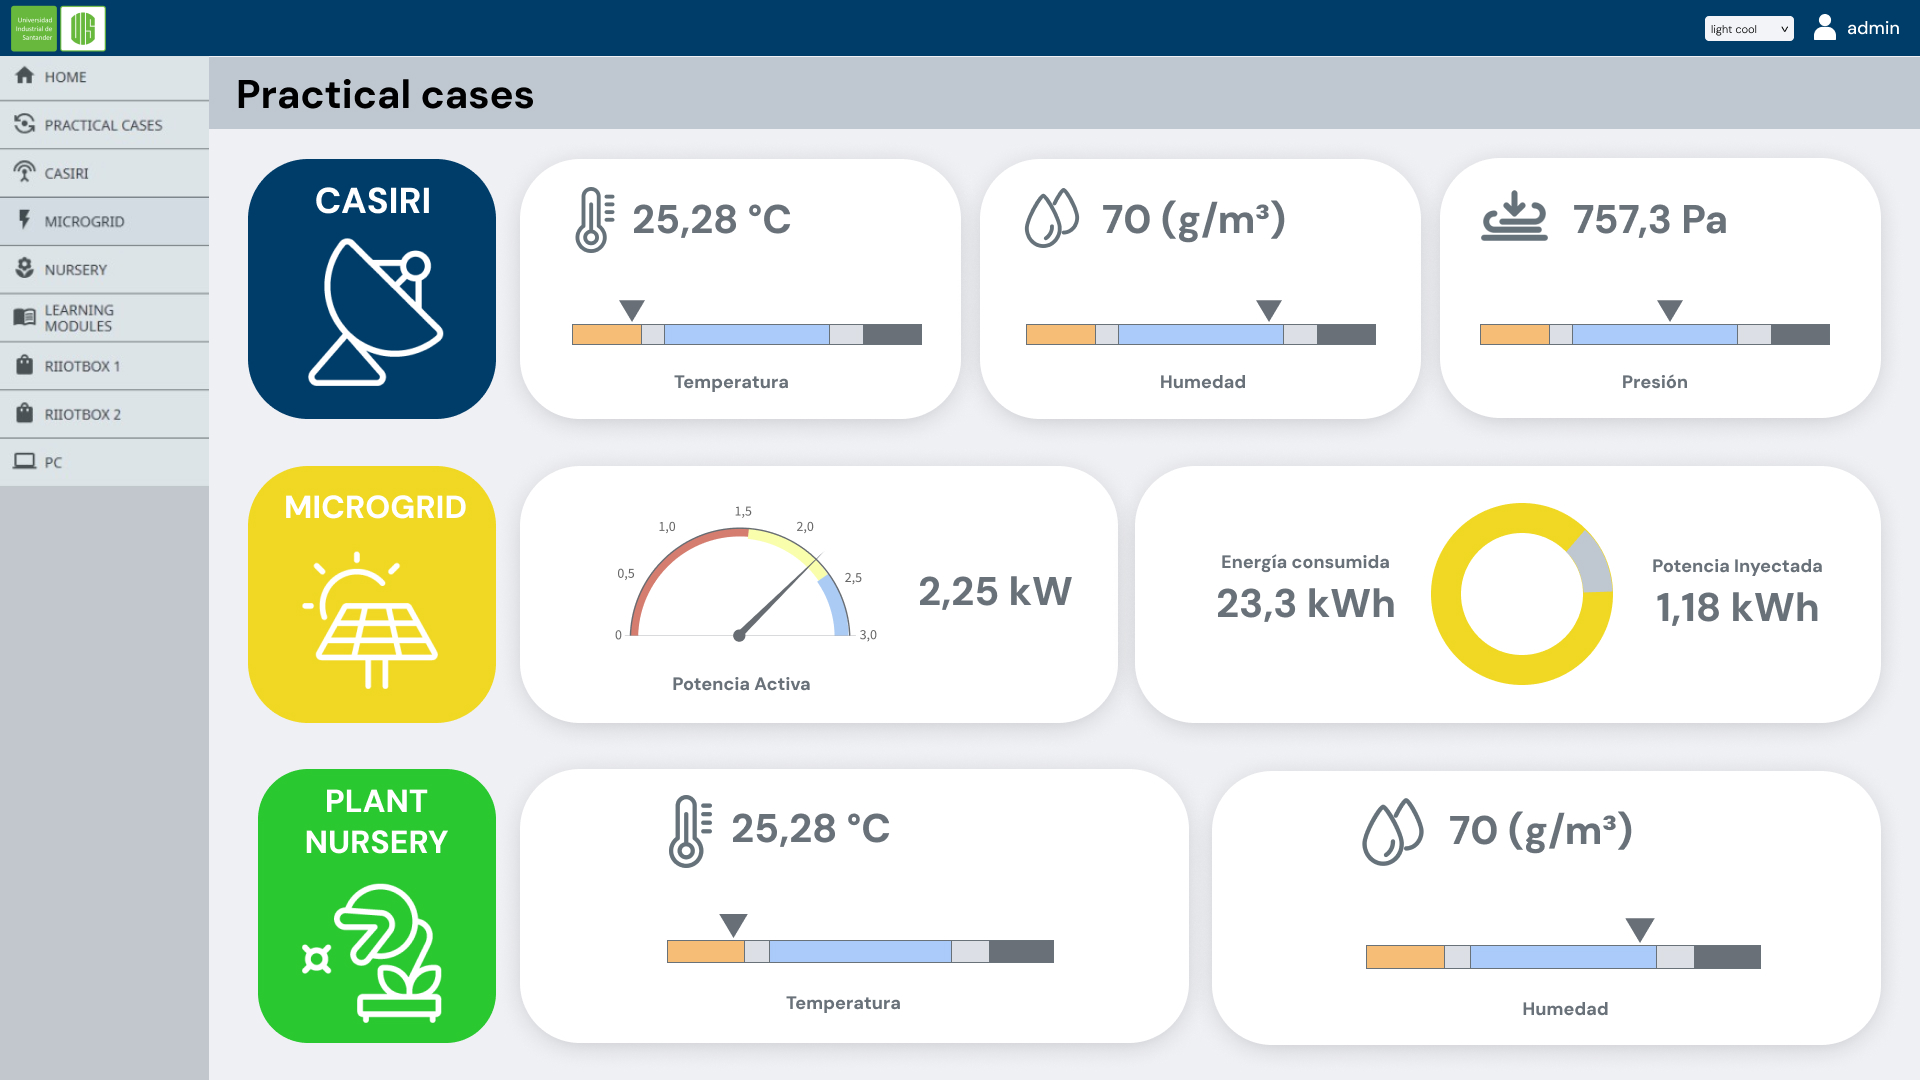
\includegraphics[width=15cm]{Figuras/HomeUNS}}
\caption{Vista del Home en la aplicación de Ignition}
\label{fig:homeUNS}
\end{figure}


La Figura \ref{fig:casiriView} muestra la visualización correspondiente a Casiri, dentro del área Radiogis del site Central. En esta vista, se monitorean variables ambientales capturadas por la Estación Ambiental y se obtienen las imágenes capturadas por la Cámara espectral, presentando los datos en tiempo real mediante gráficos e indicadores analógicos y datos históricos.


\begin{figure}[H]
\centerline{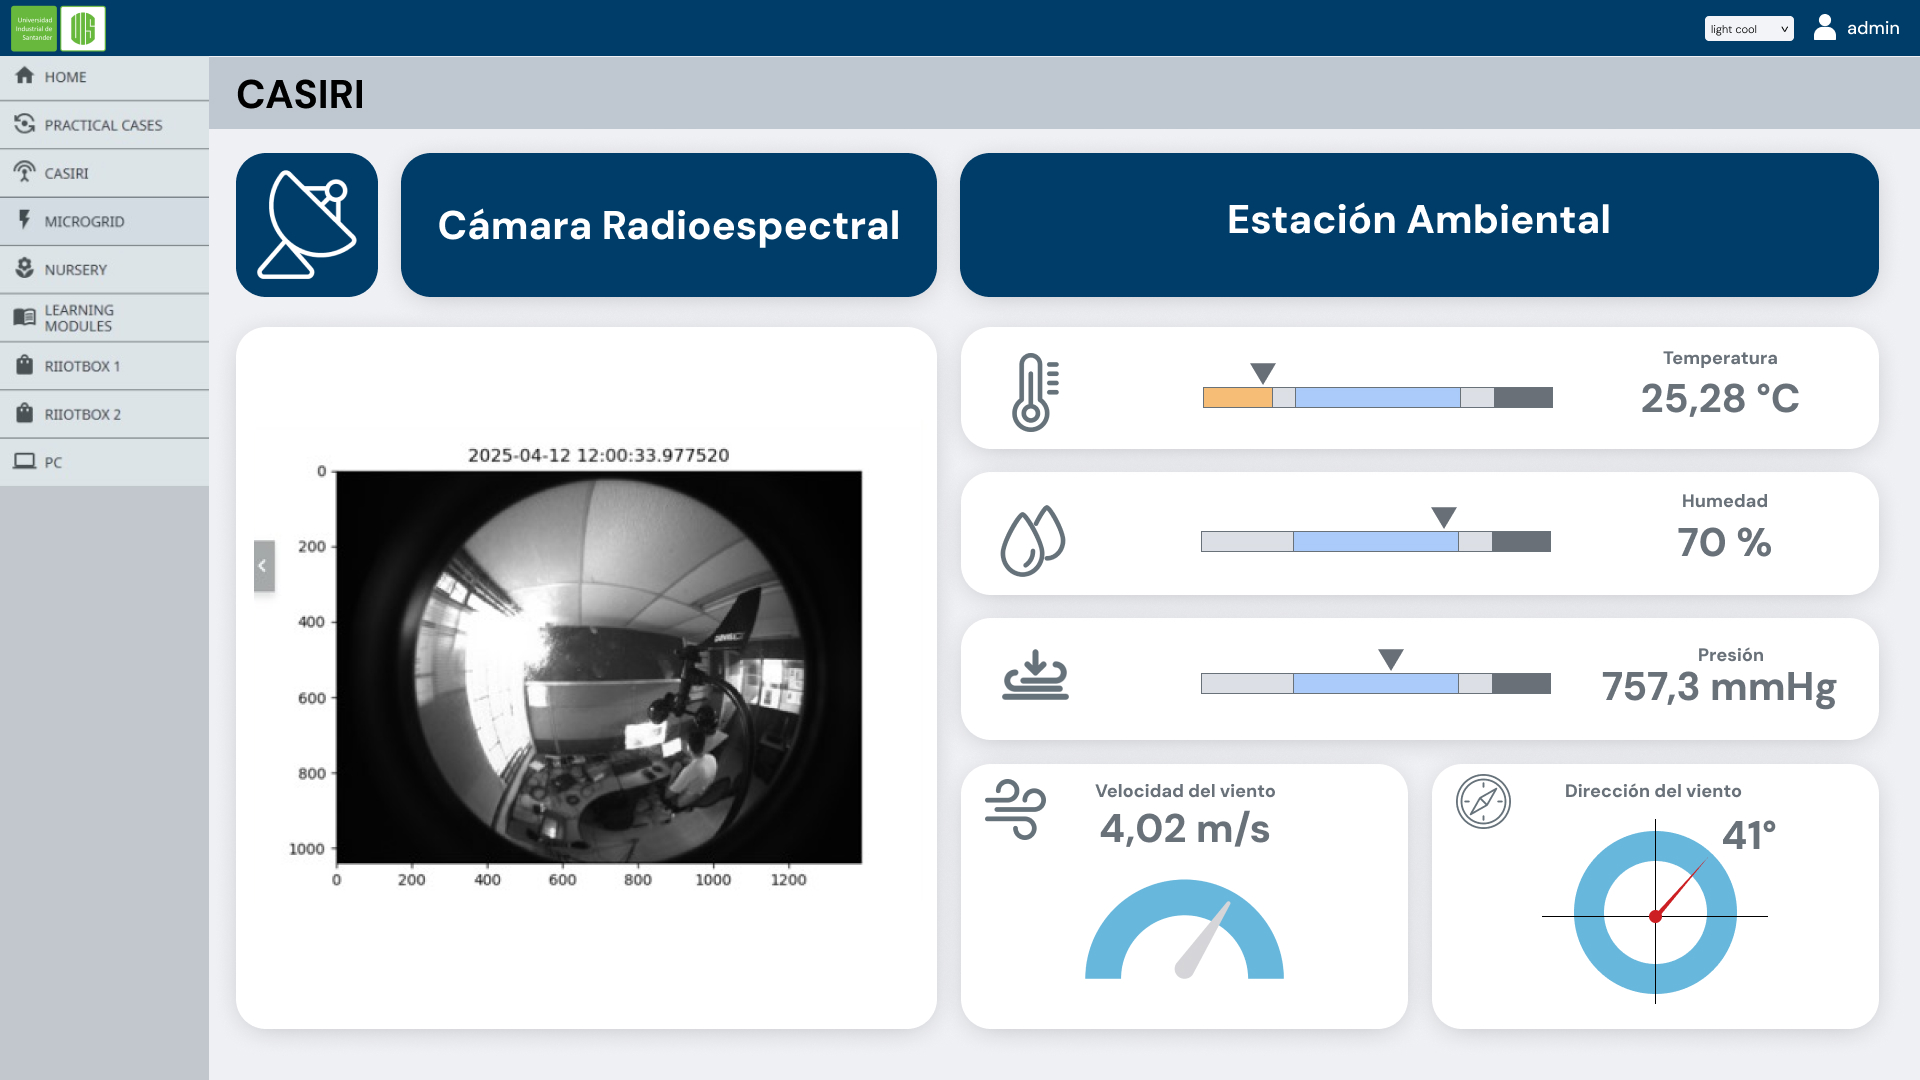
\includegraphics[width=14.1cm]{Figuras/ViewCasiri}}
\caption{Vista de Casiri en la aplicación de Ignition}
\label{fig:casiriView}
\end{figure}


En la Figura \ref{fig:microrredView}, se ilustra la vista de la Microrred, ubicada en el área LIE del site Guatiguará. Esta vista permite observar el comportamiento eléctrico de cada una de las fases de la Microrred que permite leer el PLC GroovEpic, representando variables claves del sistema.

\begin{figure}[H]
\centerline{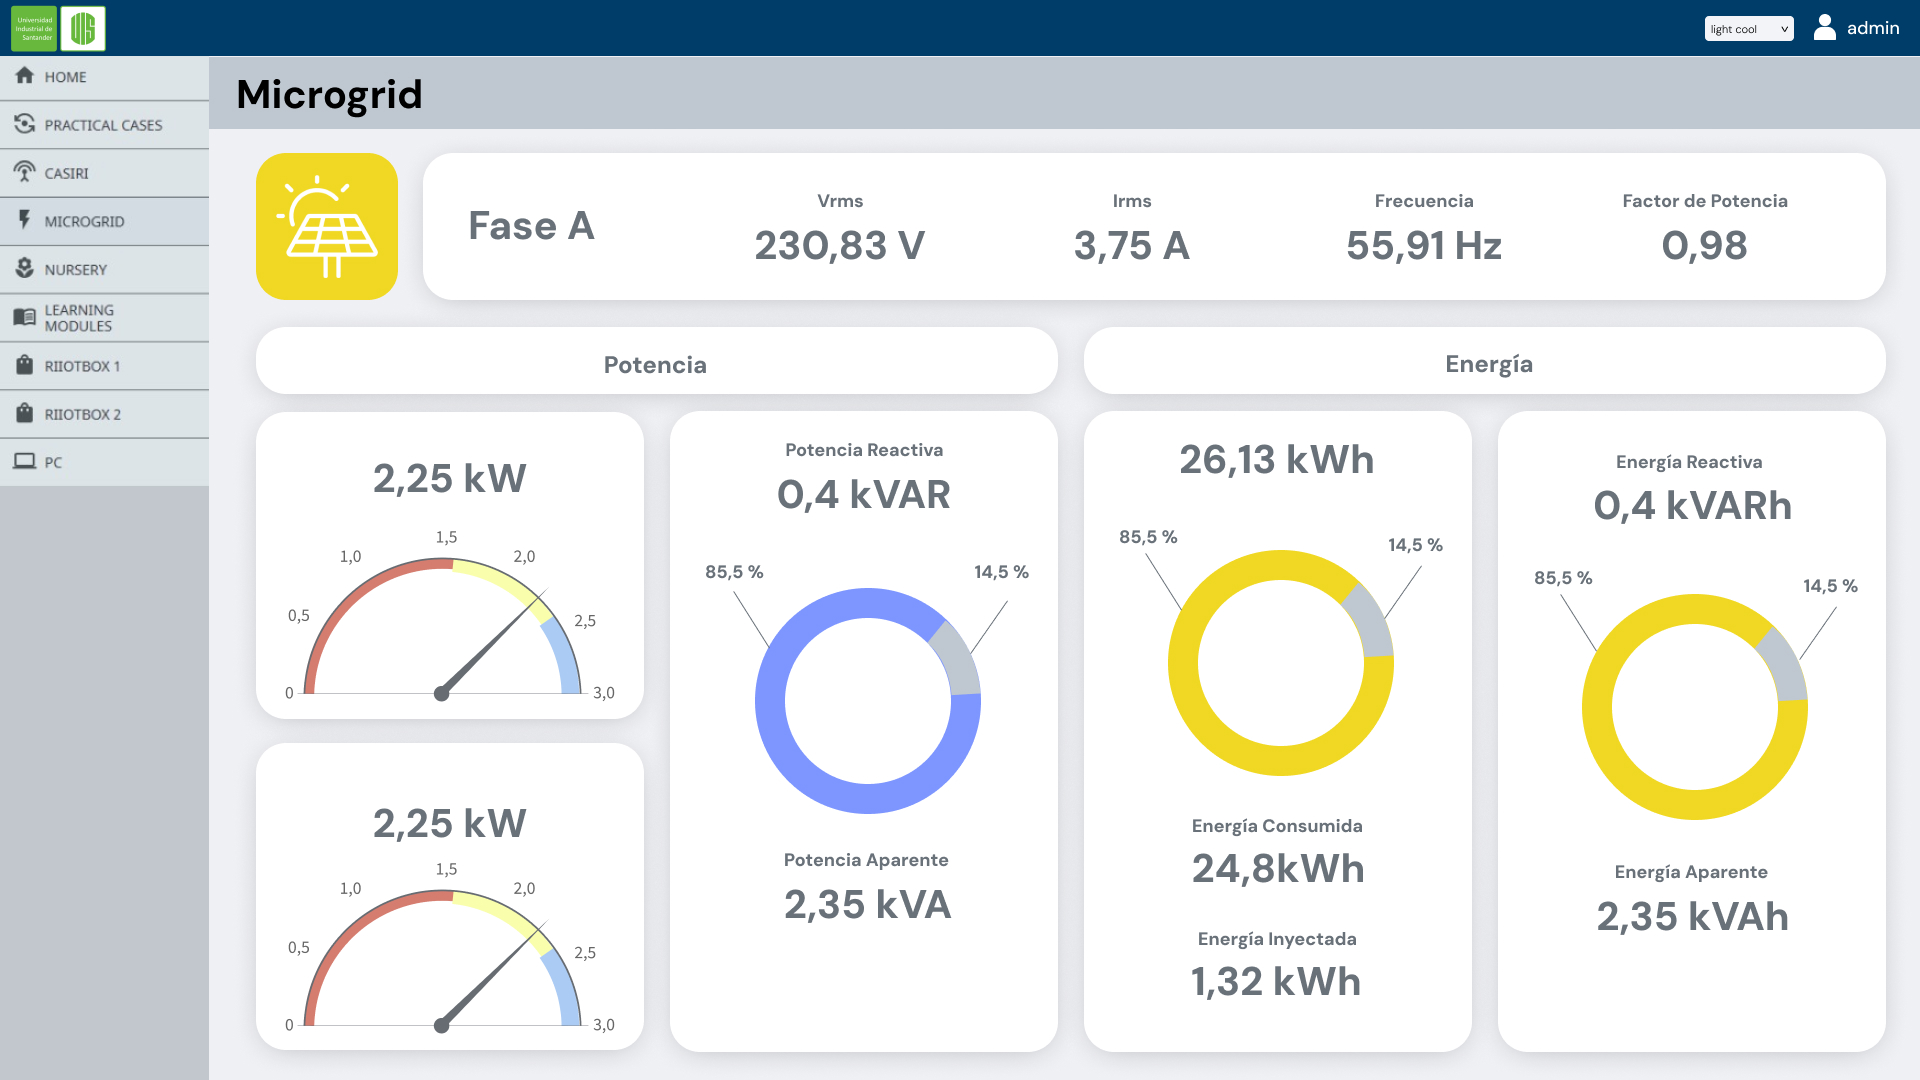
\includegraphics[width=14.1cm]{Figuras/ViewMicrorred}}
\caption{Vista de la Microrred en la aplicación de Ignition}
\label{fig:microrredView}
\end{figure}



Finalmente, la Figura \ref{fig:viveroView} corresponde a la vista del Vivero, parte del área Cenivam del site Central. En esta interfaz se visualizan parámetros ambientales recolectados por el termo-higrómetro a través del PLC GroovRio, permitiendo una supervisión detallada de las condiciones del entorno y un historial de cada una de ellas.

\begin{figure}[H]
\centerline{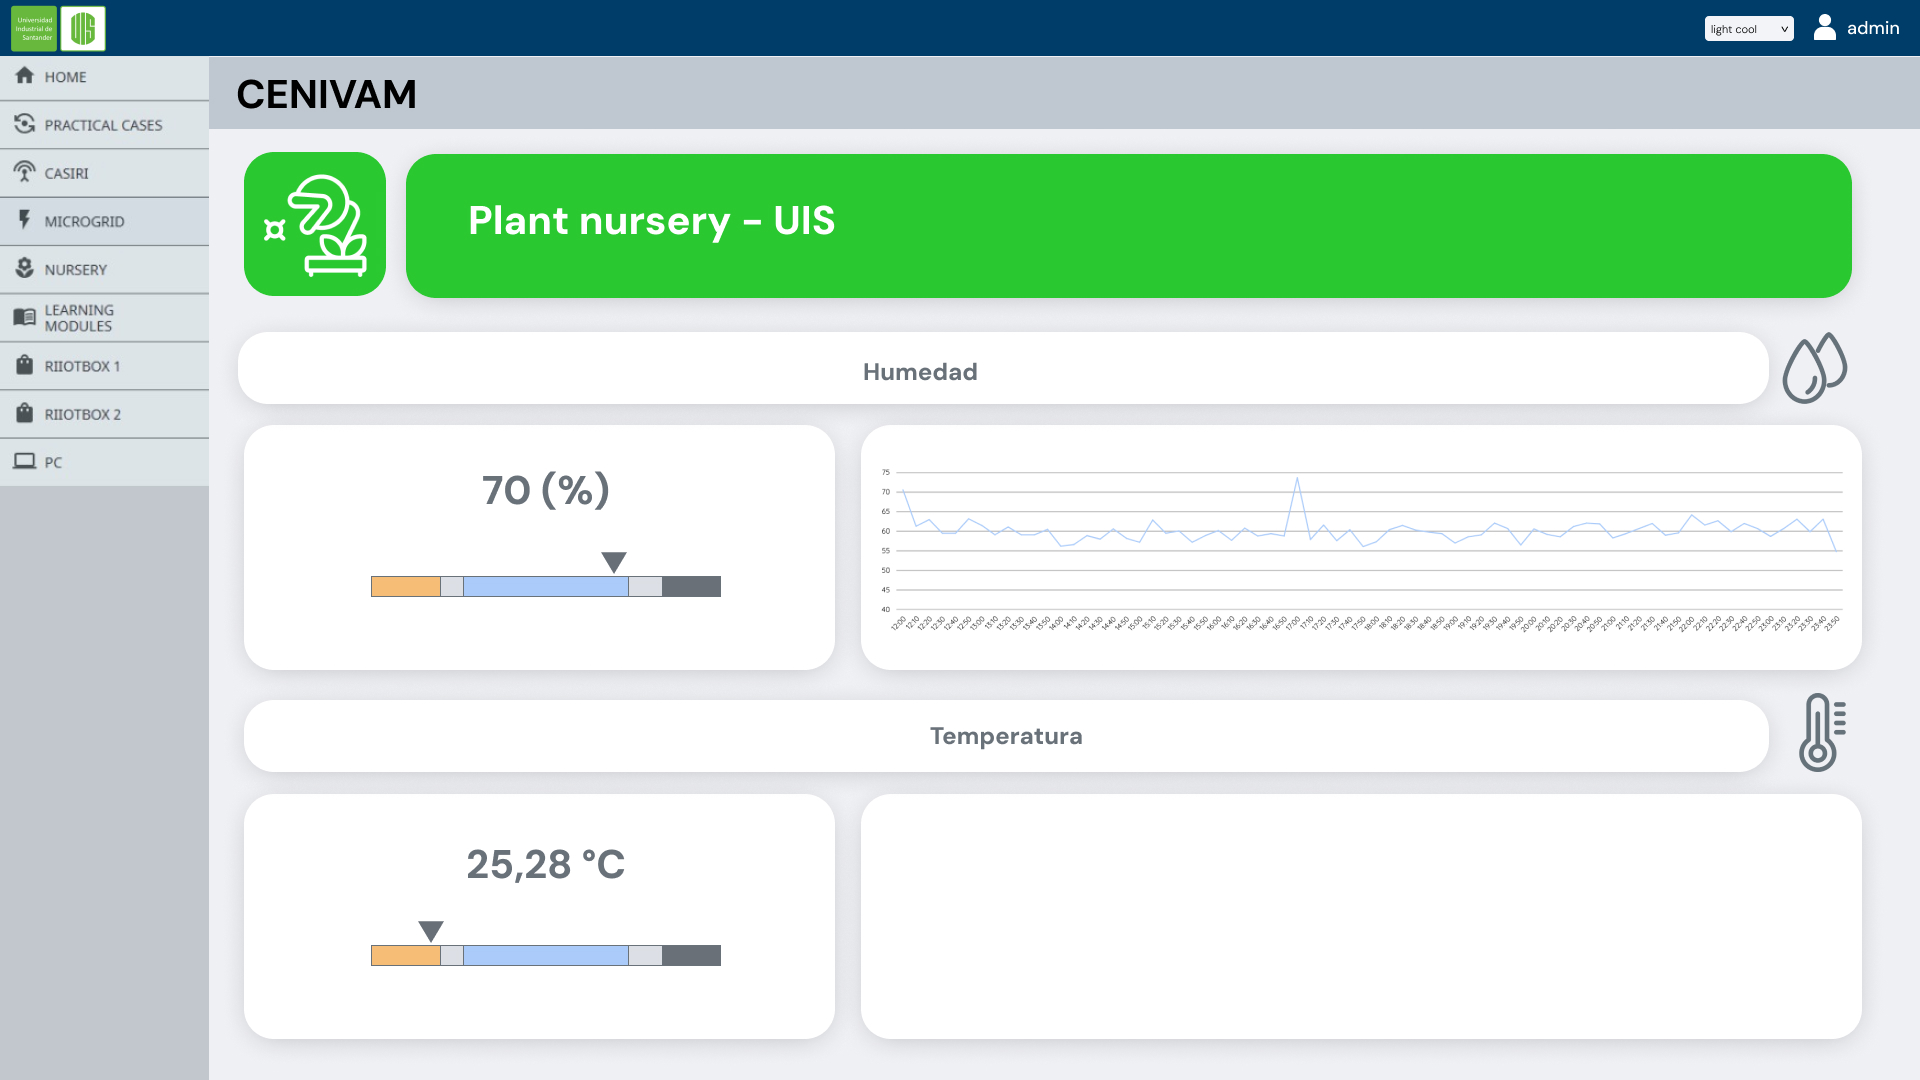
\includegraphics[width=15cm]{Figuras/ViewCenivam}}
\caption{Vista del Vivero en la aplicación de Ignition}
\label{fig:viveroView}
\end{figure}

Estas interfaces gráficas están diseñadas para ofrecer una interacción eficiente y en tiempo real entre el usuario y el sistema, permitiendo la supervisión y análisis de los datos mediante una visualización estructurada según la jerarquía definida en el UNS. La presentación contextualiza a nivel general la información proveniente de cada unos de los dispositivos integrados en cada caso de estudio dentro de la plataforma de entrenamiento IIoT.

Adicionalmente, la aplicación incorpora un mecanismo de acceso seguro basado en credenciales, lo que permite gestionar permisos según el perfil de cada usuario. La navegación se organiza mediante un árbol jerárquico que facilita el ingreso personalizado a cada una de las vistas disponibles, asegurando una experiencia flexible, escalable y orientada al rol del operador dentro del entorno industrial.






